\documentclass[11pt]{article}

% ------- Enable UTF8 characters ------- %
\usepackage[utf8]{inputenc}
\usepackage[english]{babel}

\usepackage[toc,page]{appendix}

\usepackage{listings}
\usepackage{color}
\usepackage[colorinlistoftodos]{todonotes}
%\usepackage{pdfpages}

\usepackage{epstopdf}
\usepackage{wrapfig}
\usepackage{pdfpages}
\usepackage{todonotes}
\usepackage{multicol}
\usepackage{amsmath}
\usepackage{amssymb}
% ------------ Code Listing ------------- %

\definecolor{dkgreen}{rgb}{0,0.6,0}
\definecolor{gray}{rgb}{0.5,0.5,0.5}
\definecolor{mauve}{rgb}{0.58,0,0.82}

\lstset{frame=false,
  language=VHDL,
  aboveskip=3mm,
  belowskip=3mm,
  showstringspaces=false,
  columns=flexible,
  basicstyle={\small\ttfamily},
  numbers=left,
  numberstyle=\tiny\color{gray},
  keywordstyle=\color{blue},
  commentstyle=\color{dkgreen},
  stringstyle=\color{mauve},
  breaklines=true,
  breakatwhitespace=true,
  tabsize=3,
  moredelim=**[is][\color{mauve}]{@}{@},
}

% ------- Page layout ------- %
\usepackage{fullpage}
\usepackage{hyperref} % clickable references
\hypersetup{
    colorlinks,
    citecolor=black,
    filecolor=black,
    linkcolor=black,
    urlcolor=black
}
\usepackage{multicol}
\setlength{\columnsep}{1cm}

% ------- Images ------- %
\usepackage{graphicx}
\usepackage{caption}
\usepackage{float}
\usepackage{subcaption}
\DeclareCaptionFont{gray}{\color{gray}}
\captionsetup{textfont={footnotesize,sc,gray},font={footnotesize,sc,gray}}

\usepackage{blindtext}

% Test

\usepackage{tikz}
\usetikzlibrary{shapes,arrows,shadows}
\newcommand{\mx}[1]{\mathbf{\bm{#1}}} % Matrix command
\newcommand{\vc}[1]{\mathbf{\bm{#1}}} % Vector command

\begin{document}
\begin{titlepage}
\newcommand{\HRule}{\rule{\linewidth}{0.5mm}} % Defines a new command for the horizontal lines, change thickness here

\center % Center everything on the page
 
%----------------------------------------------------------------------------------------
%	HEADING SECTIONS
%----------------------------------------------------------------------------------------

\textsc{\LARGE University of Southern Denmark}\\[1cm] % Name of your university/college
\textsc{\Large SML (F16)}\\[0.3cm] % Major heading such as course name
\textsc{\large Statistical machine learning }\\[0.3cm] % Minor heading such as course title
\vspace{0.5cm}
\begin{figure}[H]
\centering

\includegraphics[scale=1]{img/sdu-segl.png}
\end{figure}
\vspace{0.4cm}
%----------------------------------------------------------------------------------------
%	TITLE SECTION
%----------------------------------------------------------------------------------------

\HRule \\[0.4cm]
{ \huge \bfseries SML - Final Report}\\[0.4cm] % Title of your document
\HRule \\[1.5cm]
 
%----------------------------------------------------------------------------------------
%	AUTHOR SECTION
%----------------------------------------------------------------------------------------

\begin{minipage}{0.4\textwidth}
\begin{flushleft} \large
\emph{Author:}\\
Mikael \textsc{Westermann}\\
\url{miwes12@student.sdu.dk}\\
Keerthikan \textsc{Ratnarajah}\\ % Your name 
\url{kerat12@student.sdu.dk}
\end{flushleft}
\end{minipage}
~
\begin{minipage}{0.4\textwidth}
\begin{flushright} \large
\emph{Lecturer:} \\
Prof. Norbert \textsc{Krüger}\\ % Supervisor's Name
\url{norbert@mmmi.sdu.dk}
\end{flushright}
\end{minipage}\\[4cm]

% If you don't want a supervisor, uncomment the two lines below and remove the section above
%\Large \emph{Author:}\\
%John \textsc{Smith}\\[3cm] % Your name

%----------------------------------------------------------------------------------------
%	DATE SECTION
%----------------------------------------------------------------------------------------

{\large \today}\\[3cm] % Date, change the \today to a set date if you want to be precise

%----------------------------------------------------------------------------------------
%	LOGO SECTION
%----------------------------------------------------------------------------------------

%\includegraphics{Logo}\\[1cm] % Include a department/university logo - this will require the graphicx package
 
%----------------------------------------------------------------------------------------

\vfill % Fill the rest of the page with whitespace

\end{titlepage}
\tableofcontents
\newpage
\listoffigures
\newpage
\section{Introduction}
<<<<<<< HEAD
\todo[inline]{Something...}
The purpose of this report is to develop a system capable of recognizing hand writting characters such as digits (0 - 9).  This report will contain different approaches of classifying this, and their performance.  The dataset used for training and testing the performance of this, has be been made by the students of the statical machine learning class  as seen in \ref{fig:data}. The dataset consist of 400 $\times$ 10 individually handwritten numbers,  provided by each  student of the class.  

\begin{figure}[H]
\centering
\includegraphics[width =0.6\textwidth]{../../SML-database/2016/group2/member1/Ciphers100-0.png}
\caption{Example of the  dataset}
\label{fig:data}
\end{figure} 

The process of recognizing the digits can be divided into 3 steps. 
\begin{itemize}
\item Preprocessing - Extracting the data, and discard irrelevant information. 
\item Feature extraction - Extracting relevant features 
\item Classification - Use the extracted to classify the digits. 
\end{itemize}

=======
>>>>>>> 34ff1c3365fe38aae75203e9098a9fe6bb020ed5

\section{SVM}
Support vector machines is a supervised learning method that analyzes the data and tries to recognize patterns, within the classification domain. The standard SVM method is an binary classifier, which predicts for a given input which class the input belongs two. Prediction is done based on the model it builds from the training session, the model provides a "clear gap" that provide the distinction between the first or the latter class. \\

Support vector machine constructs a hyperplane or set of hyperplanes in a high dimension. The hyperplane that has the largest distance to the nearest training data points of any class (so-called functional margin), provides the best separation,  since it result it a clear distinction between the classes, and lower general error.
\\

The goal in SVM is to find this hyperplane which provides the optimal separation of the classes by having the widest margin. 

\begin{figure}[H]
\centering
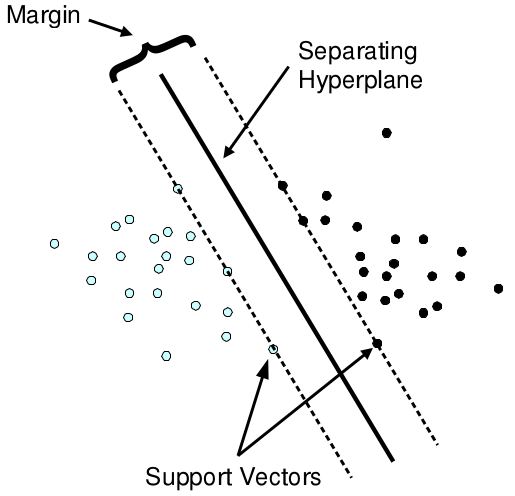
\includegraphics[width = 0.5\textwidth]{img/SVM-illu.png}
\caption{Svm Illustrated}
\label{fig::SVM-illustrated}
\end{figure}

The training data for this method consist a set of input vectors denoted as $\mathbf{x_i}$, each input vector has a number of component features. Each input vector is given a label, indicating its class.

The hyperplane is given as 
\begin{equation}
\mathbf{w} \cdot \mathbf{x} + b = 0
\end{equation}

In which the $\mathbf{w}$ determines the orientation of the plane, and $\mathbf{b}$ is the offset of the plane from the origin. \\
 
The seperaing hyperplane which maximizes the margin can be found by examining the convex hull of each class’s training data  and then find the closest points in the two convex hulls. The convex hull of a set of points is the
smallest convex set containing the points.  If the hyperplane that bisects both convex hulls can be found, will the resulting classifier deemed robust in some sense. 

\begin{figure}[H]
\centering
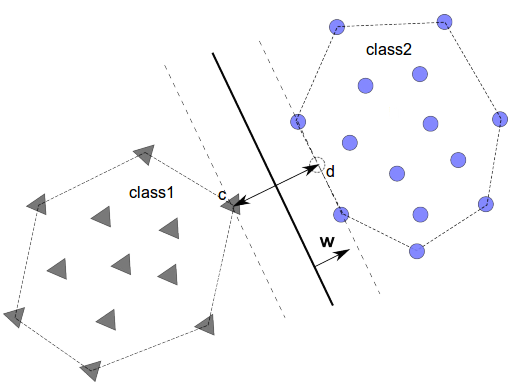
\includegraphics[width = 0.5\textwidth]{img/convex_hull.png}
\caption{best plane bisects closest points in the convex hulls,The convex hulls are labeled c and d}
\label{fig::convex_hull}
\end{figure}  

To find  the plane, one have to find the points closest to the plane, which can be found by solving the quadratic problem. \\ 

\begin{equation}
min_\alpha~\left(\frac{1}{2} ||c-d||^2\right)
\end{equation}

where c and d are the closest to be found points, these are defined as 
\begin{equation}
\begin{aligned}
&c = \sum_{y_i~\in~class1} \alpha_ix_i  
& \text{subject to}
&& \sum_{y_i~\in~class1}\alpha_i =1 
&& \alpha_i \geq 0
\end{aligned} 
\end{equation}

\begin{equation}
\begin{aligned}
&d = \sum_{y_i~\in~class2} \alpha_ix_i  
& \text{subject to}
&& \sum_{y_i~\in~class2}\alpha_i =1 
&& \alpha_i \geq 0
\end{aligned} 
\end{equation}


An alternative approach involves a search through the space of every possible hyperplane in order to find a set of two parallel planes that divide the points into homogeneous groups yet themselves are as far apart as possible.\\


In the case of non-linearly separable data, can a linear hyperplane not be used to define the solution. For this purpose is a slack variable introduced, which allows some points on the incorrect side of the margin, creating a soft margin, when a linear hyperplane was used to separate them.\\

A different approach for solving this problem would be using the kernel trick. The kernel trick involves transforming in $\mathbb{R}^n \rightarrow \mathbb{R}^{n+1}$. The challenging part is to find such transformation, $\phi$ which allow transforming data into a higher dimension. 

Kernel functions are in general in the following form:
\begin{equation}
K(\overrightarrow{x_i},\overrightarrow{x_j}) = \phi(\overrightarrow{x_i}) \cdot \phi(\overrightarrow{x_j}) 
\end{equation}

$x_i$ and $x_j$ illustrates two different feature vectors. 

Different kernels does already exist, and may already be implemented in different SVM software packages. 

\textbf{Linear kernel}:
\begin{equation}
K(\overrightarrow{x_i},\overrightarrow{x_j}) = (\overrightarrow{x_i}) \cdot (\overrightarrow{x_j}) 
\end{equation}

Linear kernel does not transform the data, but computes the dot product. 

\textbf{Polynomial kernel of degree $d$}:
\begin{equation}
K(\overrightarrow{x_i},\overrightarrow{x_j}) = ((\overrightarrow{x_i}) \cdot (\overrightarrow{x_j})+1)^d
\end{equation}

The Polynomial kernel adds a nonlinear transformation of the data.


\textbf{Sigmoid kernel}
\begin{equation}
K(\overrightarrow{x_i},\overrightarrow{x_j}) = tanh( k(\overrightarrow{x_i}) \cdot (\overrightarrow{x_j}) - \delta)
\end{equation}

The choice of kernel depends what kind of transformation is needed. 

\end{document}

